\newpage
\section{Physically Based Rendering}
% . after a mathema
It needs to be stated that the engine utilizes PBR - physically based rendering. It is a rendering technique simulating the behavior of real light rays, which can create spectacularly realistic images. Physically based rendering used to be a too complex algorithm to use in real time, like it is used in TSEngine, however, with the growing capabilities of the computers for the last decades it has become more common for real time usage of the technique in real time applications, for example in computer games.

\begin{figure}
    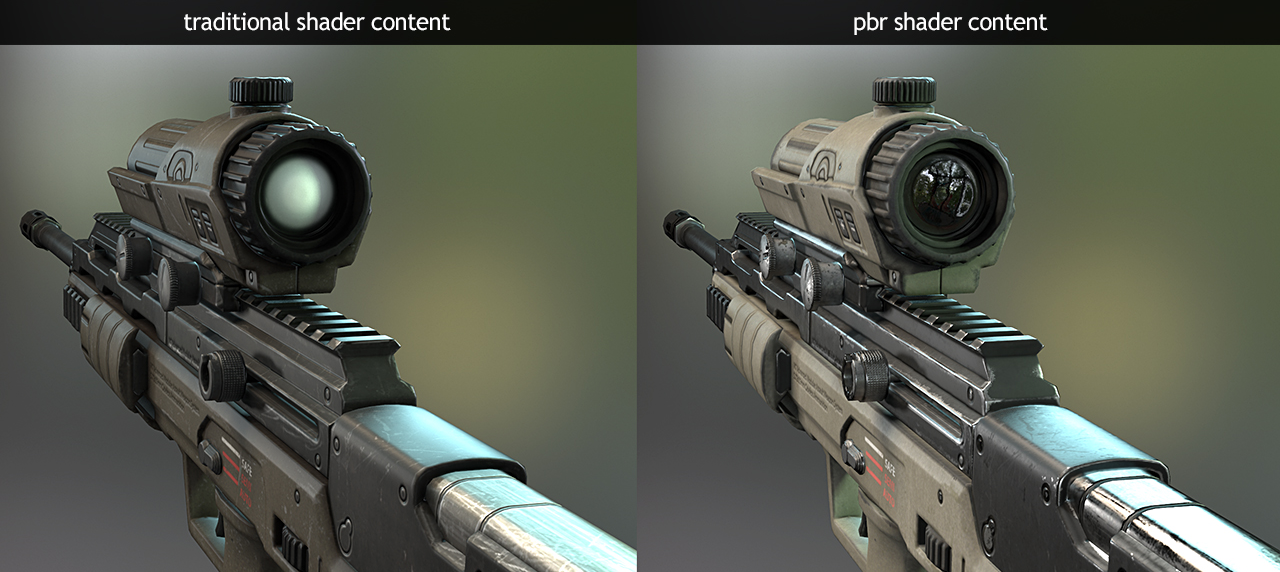
\includegraphics[width=\linewidth]{PBR-Example-Meta3DStudios.png}
    \caption{Example of PBR from META3DStudios}
\end{figure}

Many of the nowadays implementations of the algorithm, are based on the paper from 2012, Physically Based Shading at Disney by Brent Burley, Walt Disney Animation Studios. This work accumulates much of the knowledge from studies made on PBR since 1960s and builds on it. Its main defining feature is the usage of the BRDF - bidirectional reflective distribution function, which takes the incoming ($\omega i$) and outgoing ($\omega o$) directions, normal (n) of the surface and different parameters defining the surface's properties. TSEngine only takes the surface's roughness as a parameter and uses Cook-Torrance specular bidirectional reflective distribution function, which is defined as follows:
\begin{equation}
f_{CookTorrance}=\frac{DFG}{4(\omega_{O} \cdot n)(\omega_{i} \cdot n)}
\text{ .}
\label{wzor1}
\end{equation}
jygy
\begin{equation}
f_{CookTorrance}=\frac{DFG}{4(\omega_{O} \cdot n)(\omega_{i} \cdot n)}
\text{ .}
\end{equation}
As one can see the function is composed of three functions D, F and G and a normalization factor. Each of the three functions is responsible for approximating specific part of the surface's reflective properties:\\
D - Normal distribution function, responsible for ..... \\
F - Fresnel equation, which ......\\
G - Geometry function describing......
\ref{wzor1}

% Refactor
The Cook-Torrance specular BRDF is composed of three functions and a normalization factor in the denominator. Each of the D, F and G symbols represent a type of function that approximates a specific part of the surface's reflective properties. These are defined as the normal Distribution function, the Fresnel equation and the Geometry function:\\
Normal distribution function: approximates the amount the surface's microfacets are aligned to the halfway vector, influenced by the roughness of the surface; this is the primary function approximating the microfacets.\\
Geometry function: describes the self-shadowing property of the microfacets. When a surface is relatively rough, the surface's microfacets can overshadow other microfacets reducing the light the surface reflects.\\
Fresnel equation: The Fresnel equation describes the ratio of surface reflection at different surface angles.

Based on the book Learn OpenGL \cite{learnopengl} and the article \cite{pbrreferences}